
\section{Further Environment Details} \label{sec:environment_details}
The replayed data was mainly recorded or simulated  in the time from 07.01.2007 to 28.12.2008. Although some episodes had to be left out due to missing data, there were more than 100 episodes, of which 95 were supposed to be used for training, 4 for testing and the rest for evaluation. The power was standardized to kilowatts and the energy respectively to kWh. The location of the house was in France near Paris.
\par
The carbon intensity data was only available from 2021 and 2022 for France, so the carbon intensity might be biased since the electricity mix might have drifted over the years. However, the daily, weekly and yearly frequencies should still be captured, although potentially drifted. The unit of carbon intensity is grams of CO\textsubscript{2} equivalent emissions per kWh.
\par To prevent the ESS from overcharging or overdischarging, the rates were further constrained by the current charge and capacity, such that actually $C_t \in [0, \min\{C_{max}, \frac{B_{max} - B_t + D_s}{\sqrt{\nu}}\}]$ and $D_t \in [0, \min\{D_{max}, (B_t - D_S) \sqrt{\nu}\}]$.

\section{Thresholding Baseline} \label{sec:thresholding_baseline}
\begin{equation}
    a_t = \left\{
        \begin{array}{ll}
            \begin{bmatrix} \phantom{-}1 & [1]^H & \psi \end{bmatrix} & \text{if } I_t < \phi_1 \\
            \begin{bmatrix} -1 & [0]^H & \psi \end{bmatrix} & \text{if } I_t > \phi_2 \\
            \begin{bmatrix} \phantom{-}0 & [0]^H & \psi \end{bmatrix} & \text{else,}
        \end{array}
    \right.
\end{equation}
where $\phi_1 = 65 \frac{g}{kWh}$ and $\phi_2 = 85 \frac{g}{kWh}$ are the lower and upper threshold respectively, while 
\begin{equation}
    \psi = sign(\frac{T_{max}+T_{min}}{2} - T_{t}) clip(\frac{T_t-\frac{T_{max}+T_{min}}{2}}{1.3},0,1).
\end{equation}

\section{SAC}\label{sec:sac}
SAC is a squashed Gaussian policy, that employs entropy regularization, which adds a bonus reward in each time step proportional to the current entropy of the policy in an aim to encourage exploration. Furthermore, two Q-functions are learned and their minimal estimate is used to update the policy. The objective for SAC is
\begin{equation}
    \max _\theta \underset{\substack{s \sim \mathcal{D} \\ \xi \sim \mathcal{N}}}{\mathbb{E}}\left[\min _{j=1,2} Q_{\phi_{\hat{j}}}\left(s, \tilde{a}_\theta(s, \xi)\right)-\alpha H(\pi_\theta \mid s)\right],
\end{equation}
where $\theta$ denotes the policy parameter, $\xi$ normal Gaussian noise, $\tilde{a}_\theta(s, \xi)$ the action sampled from the current policy, $\alpha$ the entropy regularization coefficient, and $H(\pi_\theta \mid s) = \log \pi_\theta\left(\tilde{a}_\theta(s, \xi) \mid s\right)$ the entropy of the policy. The action samples are obtained as $\tilde{a}_\theta(s, \xi) = tanh(\mu_\theta(s)+\sigma_\theta(s) \odot \xi)$.


\section{PPO}\label{sec:ppo}
PPO is a trust-region based policy gradient method, which solves a constrained policy update policy via SGD. It achieves the trust region remarkably simple, by employing the following update objective:
\begin{flalign}
    \theta_{k+1} &= \arg \max _{\theta} \underset{\substack{s \sim \mathcal{D} \\ a \sim \pi_{\theta_k}}}{\mathbb{E}} \left[ L(s,a)\right]&& \\
    L(s,a)&=\min \left(\left|\frac{\pi_\theta(a \mid s)}{\pi_{\theta_k}(a \mid s)}\right|, 1\pm \epsilon \right) A^{\pi_{\theta_k}}(s, a),&&
\end{flalign}
where $A^{\pi_{\theta_k}}(s, a)$ is the advantage of the current policy, and $\epsilon$ the trust region hyperparameter, clipping the update size. Alternatively, PPO can also be implemented using a KL-divergence constraint.


\section{Training Procedure} \label{sec:training_procedure}

All experiments were run for 2000 episodes with fixed initial conditions, this took around 4 hours per algorithm on one RTX 2060 super. The training parameters are shown in \cref{tab:training_parameters}. 
\begin{table}[H]
\caption{Training Parameters}
\label{tab:training_parameters}
\vskip 0.15in
\begin{center}
\begin{small}
\begin{sc}
\begin{tabular}{lr}
\toprule
Parameter & Value\\
\midrule
$B_{max}$ & 13.5 \\
$C_{max}$ & 1 \\
$D_{max}$ & 1 \\
$\nu$ & 0.95 \\
$D_s$ & 0.01 \\
$B_0$ & 0 \\
$H$ & 25 \\
$\beta$ & 20 \\
$\delta$ & 5 \\
$T_{0}$ & 20 \\
$T_{b,0}$ & 20 \\
$r_{a}$ & 0.04 \\
$r_{b}$ & 0.1 \\
$r_{h}$ & 0.05 \\
$q$ & 0.05 \\
$L_{TCL}$ & 5 \\
$T_{max}$ & 23 \\
$T_{min}$ & 18 \\
\bottomrule
\end{tabular}
\end{sc}
\end{small}
\end{center}
\vskip -0.1in
\end{table}
For the stacked carbon intensity, the next 3 hours of carbon intensity were given in the observable too.
\par
For the eased exploration setting, the fdr observations were also only reported as a sum and no longer indiviudally.

\section{Split Reward}\label{sec:split_reward}
\begin{flalign}
    r_{noise} &= I_t (G_t - L_t) && \\
    r_{ESS} &= I_t (D_t - C_t) && \\
    r_{FDR} &= I_t (-\sum_{p \in U_e} p_r - \sum_{p \in U_d} \frac{2p}{H-1}) && \\
    r_{TCL} &= I_t (-\frac{1}{r_h} L_{TCL} a_{tcl,t}) && \\ 
    r_{discomfort} &=- \delta exp(|T_t - \frac{T_{max} + T_{min}}{2}). &&
\end{flalign}
The reward for TCL was split, since maintaining the temperature is a very different task than minimizing the energy consumption.

\section{Stacked Carbon Intensity Details} \label{sec:stacked_carbon_intensity_details}
The carbon intensity was stacked for the next 3 hours, such that the observable became $I_t = [I_t, I_{t+1}, I_{t+2}, I_{t+3}]^H$. The resulting training curve is shown in \cref{fig:training_curve_stacked}

\begin{figure}[H]
    \centering
    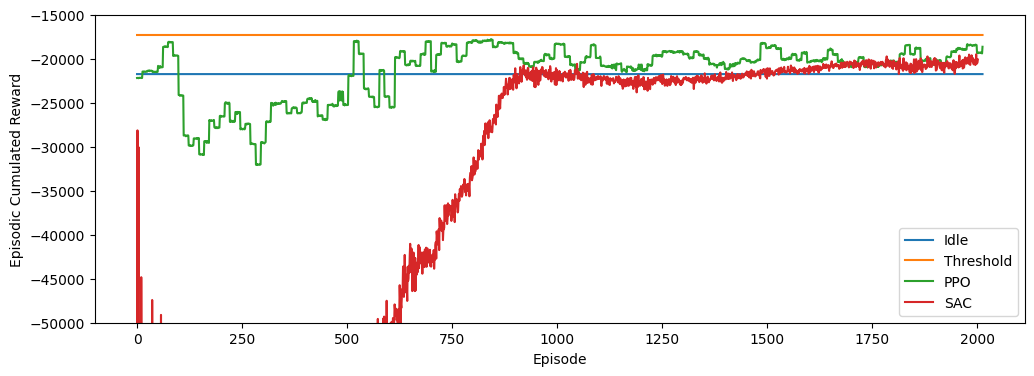
\includegraphics[width=0.85\textwidth]{figures/training_curve_stacked.png}
    \caption{Training curve for the stacked carbon intensity setting.}
    \label{fig:training_curve_stacked}
\end{figure}

\section{Eased Exploration Details} \label{sec:eased_exploration_details}
In addition to the aforementioned changes, the FDR observable was also collapsed into the scalar only reporting the sum of lined up consumptions. The training curves for the different sub-tasks are shown in \cref{fig:training_curve_scalar_ess}, \cref{fig:training_curve_scalar_fdr}, and  \cref{fig:training_curve_scalar_tcl}.
\begin{figure}[H]
    \centering
    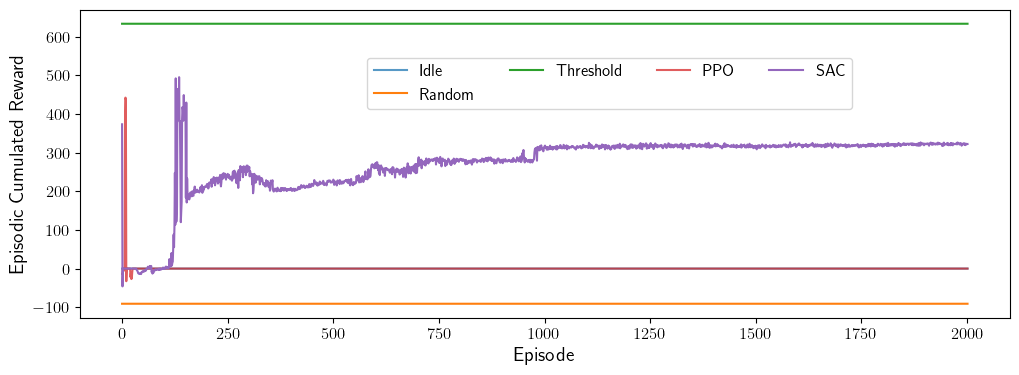
\includegraphics[width=0.85\textwidth]{figures/training_curve_scalar_ess.png}
    \caption{Training curve for ESS sub-task in the eased exploration setting.}
    \label{fig:training_curve_scalar_ess}
\end{figure}
\begin{figure}[H]
    \centering
    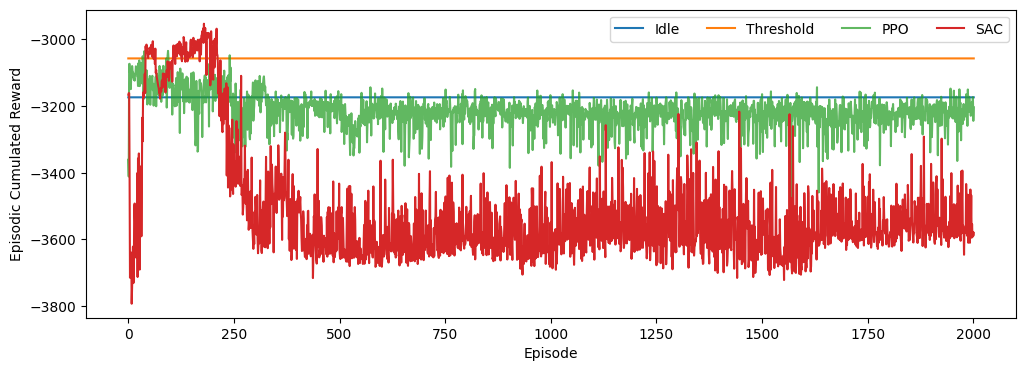
\includegraphics[width=0.85\textwidth]{figures/training_curve_scalar_fdr.png}
    \caption{Training curve for FDR sub-task in the eased exploration setting.}
    \label{fig:training_curve_scalar_fdr}
\end{figure}
\begin{figure}[H]
    \centering
    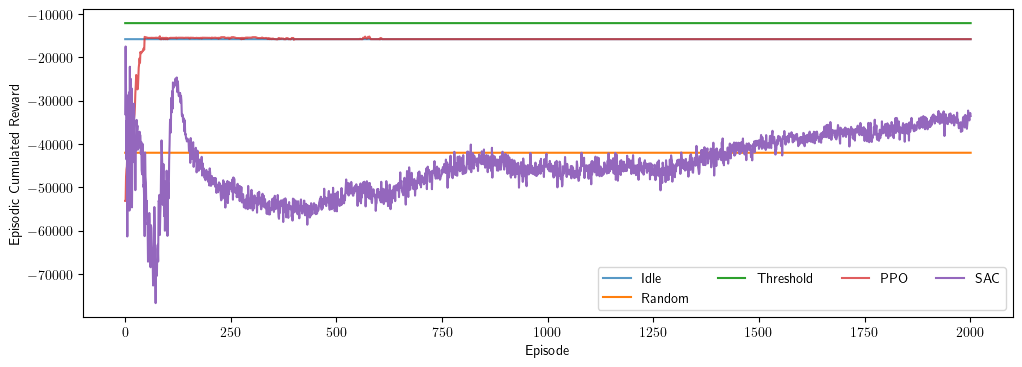
\includegraphics[width=0.85\textwidth]{figures/training_curve_scalar_tcl.png}
    \caption{Training curve for TCL sub-task in the eased exploration setting.}
    \label{fig:training_curve_scalar_tcl}
\end{figure}

\section{Terminal Reward Details} \label{sec:terminal_reward_details}
The training curve for the terminal reward setting is shown in \cref{fig:training_curve_terminal}. 
\begin{figure}[H]
    \centering
    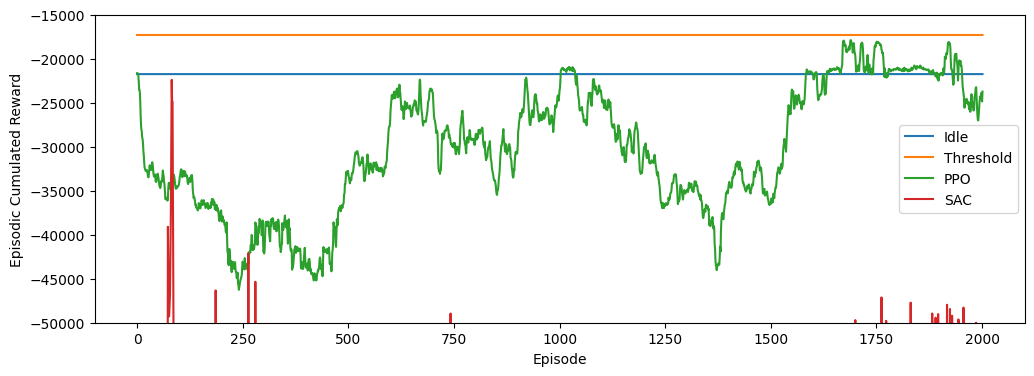
\includegraphics[width=0.85\textwidth]{figures/training_curve_terminal.png}
    \caption{Training curve for the terminal reward setting.}
    \label{fig:training_curve_terminal}
\end{figure}